\chapter{Acoustic Characteristics of Stored Product Insects in Different Materials}

Spectrograms visualize the acoustic signal as frequency magnitude over time. The following spectrograms were generated with a window size of 1024 samples and an overlap of 512 samples, resulting in an averaging of \SI{21.3}{\milli\second} time segments with a \SI{10.6}{\milli\second} step size between segments. Since the sampling frequency of the A-SPIDS system is \SI{48000}{\hertz}, the frequency resolution is \SI{46.875}{\hertz} per bin, the Nyquist frequency is \SI{24000}{\hertz}, and the maximum frequency visualized in the spectrograms is limited to \SI{12000}{\hertz}. Figure \ref{fig:darkling_beetle_spectrogram} shows the spectrograms of an example of a high strength signal, a darkling beetle, \textit{T. molitor}, in rice, from the piezoelectric channels lining the bottom of the sampling container.

\begin{figure}[!htbp]%
	\centering
	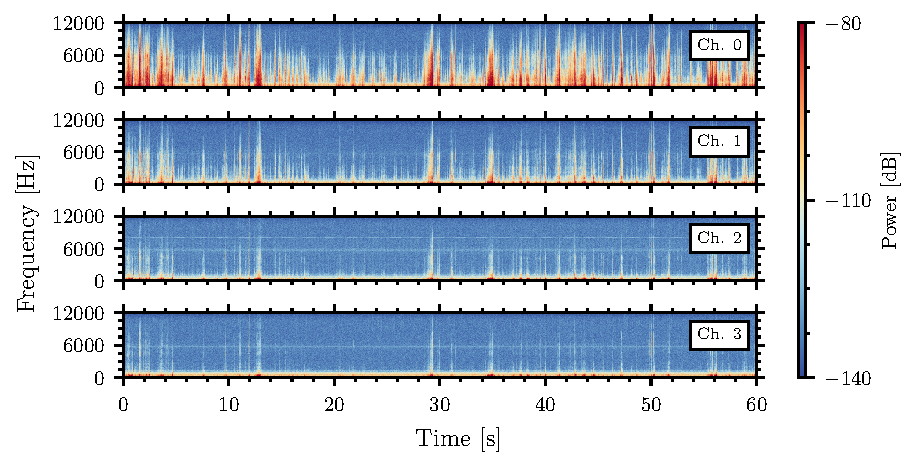
\includegraphics[width=\textwidth]{figures/1_spectrogram.pdf}
	\caption{Spectrograms from the recordings made by the internal piezoelectric channels of a darkling beetle, \textit{T. molitor}, in rice.}%
	\label{fig:darkling_beetle_spectrogram}%
\end{figure}

The impulses generated by the insect presence are clearly visible in the spectrograms as vertical lines of higher magnitude. The relatively stronger signals in channel zero indicate that the insect was located in the leftmost area of the system. The comparatively lower signal in the other channels is a result of the longer propagation distance between source and respective piezoelectric disc grouping. 

\newpage
The signal magnitude difference across the channels is verified through spectral plots, which show a snapshot of the frequency content magnitude averaged over the recording duration. Figure \ref{fig:darkling_beetle_spectra} displays the spectra generated with a 1024 sample Blackman-Harris window averaged over a \SI{60}{\second} recording of the \textit{T. molitor} in rice example compared to the reference noise produced by the sensor self-noise when no insect is present.

\begin{figure}[!htbp]%
	\centering
	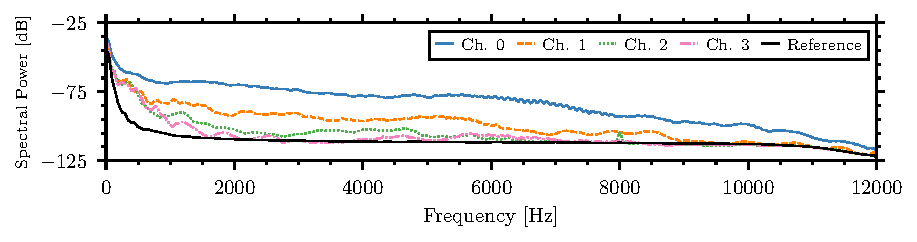
\includegraphics[width=\textwidth]{figures/2_spectra.pdf}
	\caption{Spectra from the recordings made by the internal piezoelectric channels of a darkling beetle, \textit{T. molitor}, in rice.}%
	\label{fig:darkling_beetle_spectra}%
\end{figure}

Figure \ref{fig:cfb_flour_bb_oatmeal} shows the spectrograms of the confused flour beetle, \textit{T. confusum}, in flour and the bean beetle, \textit{C. maculatus}, in oatmeal as examples of a medium and low strength signal, respectively. Only the spectrograms of the piezoelectric channels with the highest signal strength are visualized.

\begin{figure}[!htbp]
	\centering
	\begin{subfigure}{\textwidth}
		\centering
		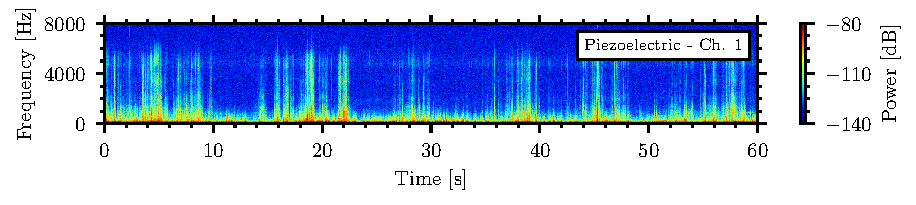
\includegraphics[width=\textwidth]{figures/acoustic_signatures/Bean beetle_Oatmeal_spectrogram.pdf}
		\caption{\textit{C. maculatus} in oatmeal}
		\label{fig:bb_oatmeal}
	\end{subfigure}%
	\qquad
	\begin{subfigure}{\textwidth}
		\centering
		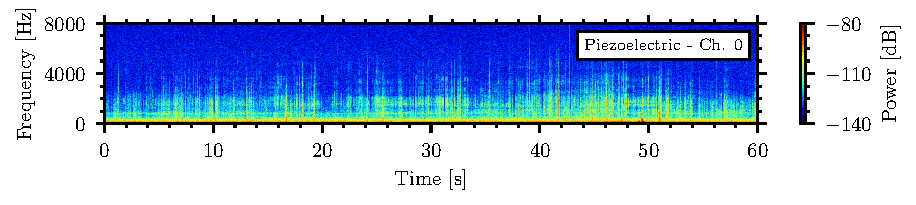
\includegraphics[width=\textwidth]{figures/acoustic_signatures/Confused flour beetle_Flour_spectrogram.pdf}
		\caption{\textit{T. confusum} in flour}
		\label{fig:cfb_flour}
	\end{subfigure}%

	% \qquad
	\caption{Spectrograms of \textit{C. maculatus} in oatmeal and \textit{T. confusum} in flour}%
	\label{fig:cfb_flour_bb_oatmeal}
\end{figure}

Figure \ref{fig:spectra} compares the spectral content of the high, medium, and low strength signals to the reference noise:

\begin{figure}[!htbp]
	\centering
	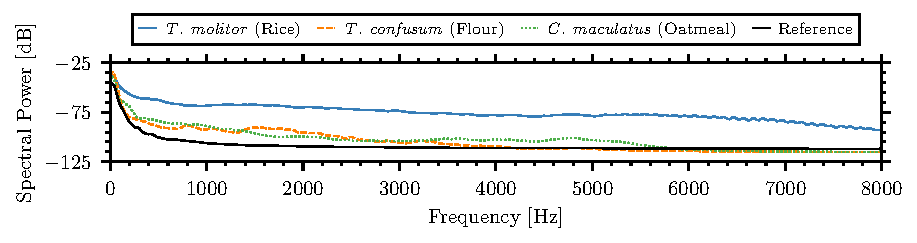
\includegraphics[width=\textwidth]{figures/acoustic_signatures/spectra.pdf}
	\caption{Comparison of the spectral content of high, medium, and low strength signals.}
	\label{fig:spectra}
\end{figure}

In these examples, the pulses that propagated to the nearest sensor had the maximal amplitude and spectral content relative to their counterparts which recorded weaker signals. Although the system lid was closed during the recording so insect location could not be verified. Based on insect behavior, it is expected that the insects remained on the surface of the substrate where the minimum distance to center of the nearest piezoelectric sensor would be \SI{5}{\centi\meter}.

\newpage
The differences between the spectra of the insect signal and the reference noise of the respective channel can be interpreted as the signal-to-noise ratio (SNR). Figure \ref{fig:snr} compares the SNR of the \textit{T. molitor} in rice, \textit{T. molitor} larva in wheat groats, \textit{T. confusum} in flour, and \textit{C. maculatus} in oatmeal to the reference noise of the respective channel.

\begin{figure}[!htbp]
	\centering
	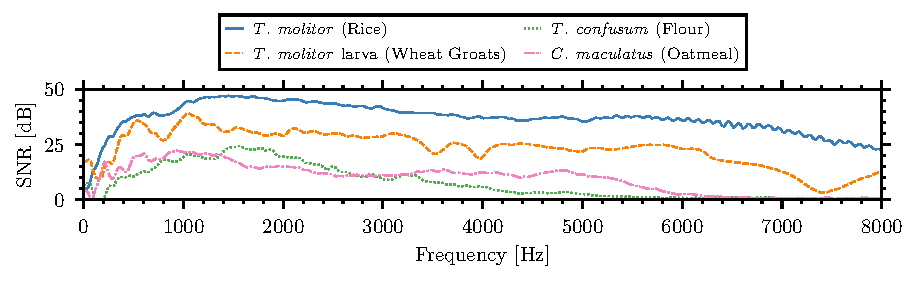
\includegraphics[width=\textwidth]{figures/acoustic_signatures/snr.pdf}
	\caption{Signal-to-Noise Ratio (SNR) of the example insect-material pairings}
	\label{fig:snr}
\end{figure}

The SNR in the presented examples is above zero in the frequency band from \SIrange{500}{6000}{\hertz}. This bandwidth was chosen for the signal analysis in the time domain during statistical comparison of the insect signal amplitude and energy for the various insects and materials when no external noise is present.

The Butterworth bandpass filter enables the extraction of the insect signal features within this frequency band \cite{parksDigitalFilterDesign1987}. Equation \ref{eq:bandpass} describes the magnitude response function of this filter:

\begin{equation}
	\label{eq:bandpass}
	M(\omega) = \frac{1}{\sqrt{1+(\frac{\omega_c^2-\omega^2}{\omega \cdot \omega_\Delta})^{2n}}}
\end{equation}

\begin{equation*}
	\omega_c = \sqrt{\omega_1 \cdot \omega_2} \qquad \omega_\Delta = \omega_2 - \omega_1
\end{equation*}

where $\omega_c$ is the center frequency, $\omega_1$ and $\omega_2$ are the lower and higher angular frequencies, respectively, and $n$ is the order of the filter \cite{vanvalkenburgAnalogFilterDesign1982}. Figure \ref{fig:butterworth} shows the waveform of the signal for \textit{T. molitor} larva in wheat groats with a \SIrange{500}{6000}{\hertz} Butterworth 10th order bandpass filter applied.

\begin{figure}[!htbp]
	\centering
	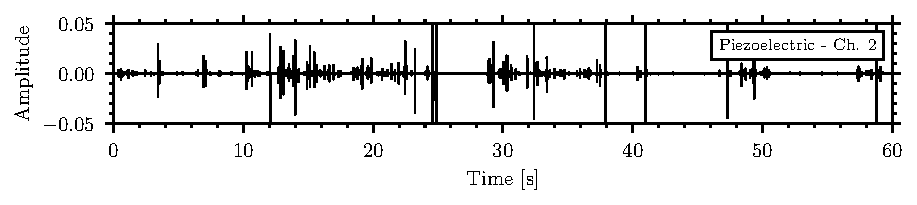
\includegraphics[width=\textwidth]{figures/acoustic_signatures/Mealworm_Wheat Groats_waveform_filtered.pdf}
	\caption{Waveform of the filtered signal for \textit{T. molitor} larva in wheat groats}
	\label{fig:butterworth}
\end{figure}

\newpage
The insect impulses can be further exposed through the envelope in the time domain. The Hilbert transform, $H$, of the signal $S(t)$ is defined in Equation \ref{eq:hilbert}:

\begin{equation}
	\label{eq:hilbert}
	\hat{S}(t) = H\{S(t)\} = \frac{1}{\pi} \int_{-\infty}^{\infty} \frac{S(\tau)}{t-\tau} d\tau
\end{equation}

where $t$ is the time and $\tau$ is the integration variable. Equation \ref{eq:analytical} shows the analytical signal, $Z(t)$, obtained by combining the original signal with the Hilbert transform:

\begin{equation}
	\label{eq:analytical}
	Z(t) = S(t) + i \hat{S}(t)
\end{equation}

The envelope of the signal is then calculated by taking the magnitude of the analytical signal, $Z(t)$, as shown in Equation \ref{eq:envelope}:

\begin{equation}
	\label{eq:envelope}
	S_E = | z(t) | = \sqrt{S^2+\hat{S}^2}
\end{equation}

where $S_E$ is the envelope of the signal \cite{ulrichEnvelopeCalculationHilbert2006}. Figure \ref{fig:envelope} shows the filtered waveform of the signal for \textit{T. molitor} larva in wheat groats with the envelope applied.

\begin{figure}[!htbp]
	\centering
	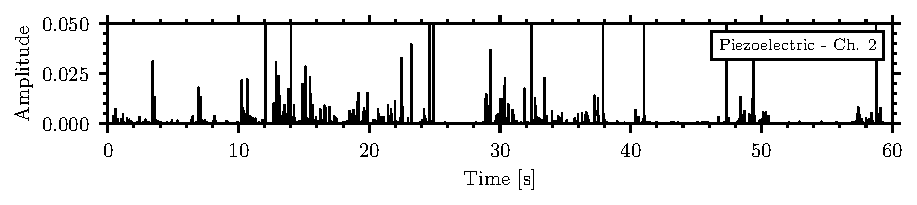
\includegraphics[width=\textwidth]{figures/acoustic_signatures/Mealworm_Wheat Groats_waveform_envelope.pdf}
	\caption{Waveform of the filtered signal for \textit{T. molitor} larva in wheat groats}
	\label{fig:envelope}
\end{figure}

The piezoelectric discs used in the A-SPIDS sensor are highly sensitive with relatively low noise levels but they are not calibrated and the recorded signals cannot be referenced with standard measurement units such as \si{\micro\pascal}, \si{\deci\bel} 20re \si{\micro\pascal}, or for acceleration in vibration measurement \si{\meter\per\second\squared}.

\section{Normalization of Signal Amplitude}

Normalization is a common practice in signal processing to adjust the amplitude of the signal to a common scale, which allows for better comparison and analysis of the signals across different sensors. The normalization process is especially important when dealing with non-calibrated sensors, as it helps to mitigate the effects of varying sensor sensitivities and external noise \cite{mainettiAcousticIdentificationWoodBoring}.

Although various publications normalize the insect amplitude for analysis, the methods are not always described in detail \todo{citations}. \citeauthor{mainettiAcousticIdentificationWoodBoring} used Z-score normalization, which standardizes every value in the collection of data so that the mean of all the values is zero and the standard deviation is one. They then applied rolling and hopping windows in order to smooth short term fluctuations and highlight trends while maintaining an improved resolution and reduce information loss at window boundaries \cite{mainettiAcousticIdentificationWoodBoring}.

Two normalization methods were implemented to accommodate for the proprietary, non-calibrated sensors. The first method uses the self-noise of the sensors as a reference. The second method was developed when self-noise records were not available and as a effective way to accommodate for influences from external noise.

\subsection{Self-noise Normalization Method}

The process of filtering and enveloping the insect signal was applied to the self-noise reference recordings for each channel. The root-mean-square (RMS) of the processed self-noise signal was then utilized as the normalization factor. Equation \ref{eq:rms} shows the calculation of the RMS value:

\begin{equation}
	\label{eq:rms}
	\text{RMS}(S) = \sqrt{\frac{1}{N} \sum_{i=1}^{N} S_i^2}
\end{equation}

where $S_i$ is the $i$-th sample of the signal $S$ and $N$ is the total number of samples in the signal. The subsequent normalization equation is presented in Equation \ref{eq:normalization}:

\begin{equation}
	\label{eq:normalization}
	S_N = \frac{S_{E, \text{BPF}(\omega_1, \omega_2)}}{\text{RMS}(N_{E,\text{BPF}(\omega_1, \omega_2)})}
\end{equation}

where the normalized signal amplitude $S_N$ is the envelope of thee bandpass filtered signal $S_{E, \text{BPF}}$ divided by the root-mean-square of the enveloped bandpass filtered reference self-noise $N_{E,\text{BPF}}$ in the frequency band from $\omega_1$ to $\omega_2$. Figure \ref{fig:normalization_diagram} shows a diagram of the signal normalization chain:

\begin{figure}[!htbp]
	\centering
	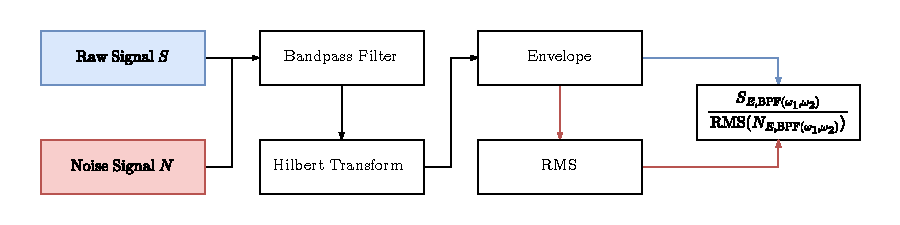
\includegraphics[width=\textwidth]{figures/normalization/normalization_process.pdf}
	\caption{Diagram of self-noise normalization process}
	\label{fig:normalization_diagram}
\end{figure}

Figure \ref{fig:normalized} shows the normalized envelope of the filtered signal for \textit{T. molitor} larva in wheat groats with the self-noise normalization method applied.

\begin{figure}[!htbp]
	\centering
	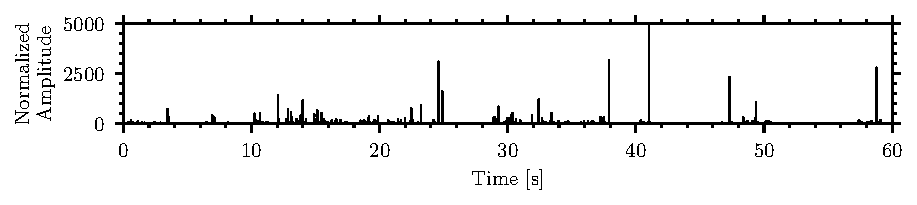
\includegraphics[width=\textwidth]{figures/normalization/Mealworm_Wheat Groats_waveform_normalized (500-6000).pdf}
	\caption{Normalized envelope of the filtered signal for \textit{T. molitor} larva in wheat groats}
	\label{fig:normalized}
\end{figure}

\subsection{Median Normalization Method}

The self-noise reference signal is an effective normalization method but requires a series of clean recordings without insects or external noise for calibration which is not always available. As an example, the BugBytes dataset does not contain recordings without insects to use as a reference signal. An alternative method to determine self-noise was developed by associating any signal below the median value of amplitude as noise. The original signal is then normalized by dividing it by the RMS of the median assumed noise signal. Equation \ref{eq:median} describes the median normalization method:

\begin{equation}
	\label{eq:median}
	S_n = \frac{S_{E,\text{BPF}(\omega_1, \omega_2)}}{\text{RMS}(N_s)} \text{ where } N_s < \text{median}(S_{E,\text{BPF}(\omega_1, \omega_2)})
\end{equation}

where the normalized signal amplitude $S_n$ is the envelope of the bandpass filtered signal $S_{E, \text{BPF}}$ divided by the root-mean-square of the noise signal $N_s$ which is any portion of the signal below the median value of the envelope in the frequency band from $\omega_1$ to $\omega_2$.

Figure \ref{fig:normalization_comparison} compares the reference signal extraction using self-noise and median noise method using the \textit{T. molitor} larva in wheat groats example.

\begin{figure}[!htbp]
	\centering
	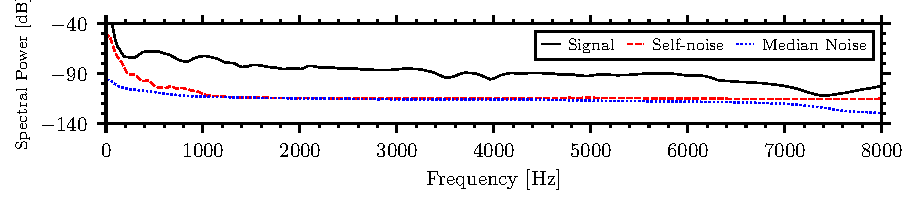
\includegraphics[width=\textwidth]{figures/normalization/normalization_comparison.pdf}
	\caption{Comparison of self-noise and median noise reference signal extraction}
	\label{fig:normalization_comparison}
\end{figure}

The median reference extraction was effective at matching the self-noise signal, especially in the 500 Hz to 6000 Hz band demonstrating that this method can be used when a clean signal is not available.

\newpage
\section{Metrics for Signal Comparison}

\subsection{Normalized Signal Pulse Amplitude (NSPA)}

% In order to compare the normalized insect signals across the different insects and materials, two metrics were derived utilizing the amplitude and spectral energy components of the respective signals.

The Normalized Strong Pulse Amplitude (NSPA) was calculated by taking the root-mean-square value of the normalized envelope within the 50\% to 90\% of the maximum and converting it to decibel amplitude. The channel with the highest NSPA was determined to be the one closest to the insect. Equation \ref{eq:nspa}  describes the calculation of the NSPA:

\begin{equation}
	\label{eq:nspa}
	\text{NSPA} = 20 \log_{10}(\text{RMS}(S_c)) \text{ where } 0.5 S_{c,\text{max}} \leq S_{c} \leq 0.9 S_{c,\text{max}}
\end{equation}

where $S_c$ is the envelope amplitude from channel $c$, RMS is the root-mean-square function, and $S_{\text{max}}$ is the maximum envelope amplitude during the analyzed record. Figure \ref{fig:nspa_graphs} shows the normalized envelopes of the insect signals in the different materials and highlights the analysis region for the NSPA calculation in red as well as distinguishes the calculated NSPA value.

\begin{figure}[!htbp]
	\centering
	\begin{subfigure}{\textwidth}
		\centering
		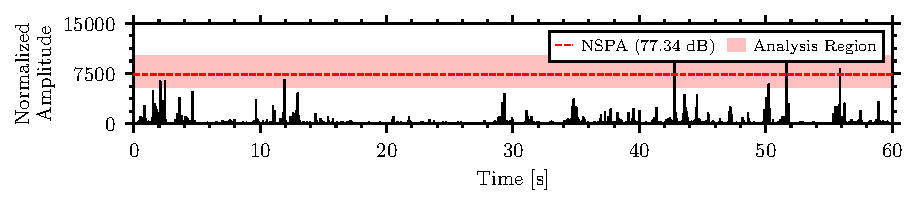
\includegraphics[width=\textwidth]{figures/nspa_nsel/Darkling beetle_Rice_nspa.pdf}
		\caption{\textit{T. molitor} in rice}
		\label{fig:nspa_tm_rice}
	\end{subfigure} \\

	\begin{subfigure}{\textwidth}
		\centering
		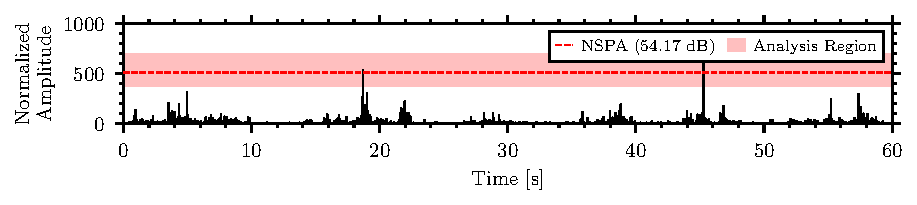
\includegraphics[width=\textwidth]{figures/nspa_nsel/Bean beetle_Oatmeal_nspa.pdf}
		\caption{\textit{C. maculatus} in oatmeal}
		\label{fig:nspa_bb_oatmeal}
	\end{subfigure} \\

	\begin{subfigure}{\textwidth}
		\centering
		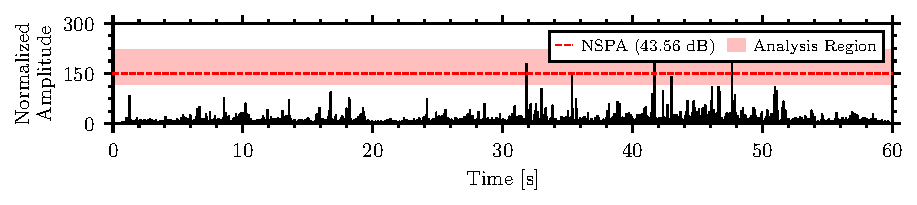
\includegraphics[width=\textwidth]{figures/nspa_nsel/Confused flour beetle_Flour_nspa.pdf}
		\caption{\textit{T. confusum} in flour}
		\label{fig:nspa_cfb_flour}
	\end{subfigure}

	\caption{Normalized Signal Pulse Amplitude (NSPA) for different insect species in various materials}%
	\label{fig:nspa_graphs}
\end{figure}

\newpage
\subsection{Normalized Spectral Energy Level (NSEL)}

The second parameter used for comparison is the Normalized Signal Energy Level (NSEL) in the frequency band \SIrange{500}{6000}{\hertz}. The total energy of the signal in the frequency band was calculated from the power spectral density (PSD), examples of which are presented in Figure \ref{fig:spectra}. This procedure is equivalent to the calculation of the sound pressure level (SPL) in a definite frequency band \cite{tachibanaDefinitionMeasurementSound1987}. Similarly to the amplitude normalization, the NSEL is then normalized to the sound pressure level of the reference noise level in the same frequency band. Equation \ref{eq:nsel} describes the calculation of the NSEL:

\begin{equation}
	\label{eq:nsel}
	\text{NSEL} = \text{SPL}(\omega_1,\omega_2) - \text{SPL}_{\text{noise}}(\omega_1,\omega_2)
\end{equation}

where $\text{SPL}(\omega_1,\omega_2)$ is the sound pressure level in the frequency band from $\omega_1$ to $\omega_2$, and $\text{SPL}_{\text{noise}}(\omega_1,\omega_2)$ is the sound pressure level of the noise in the same frequency band.

\subsection{Comparison of NSPA and NSEL}

Figure \ref{fig:nspa_nsel} shows the distribution the NSPA and NSEL for the different insect and material pairings in a box plot. The box plot centers on the median value of the insect pulses in the respective material and the extents are the 25th and 75th percentiles.

\begin{figure}[!htbp]
	\centering
	\begin{subfigure}{\textwidth}
		\centering
		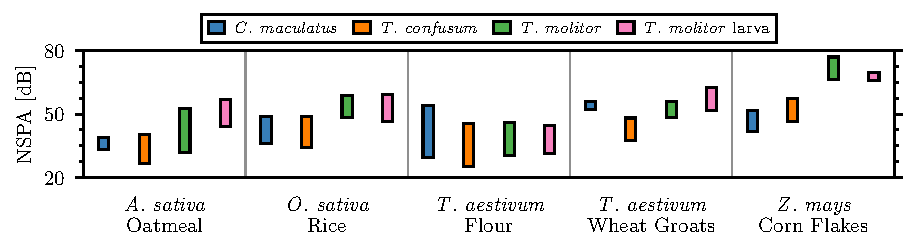
\includegraphics[width=\textwidth]{figures/nspa_nsel/nspa_box.pdf}
		\caption{Normalized Signal Pulse Amplitude (NSPA)}
		\label{fig:nspa_box}
	\end{subfigure} \\

	\begin{subfigure}{\textwidth}
		\centering
		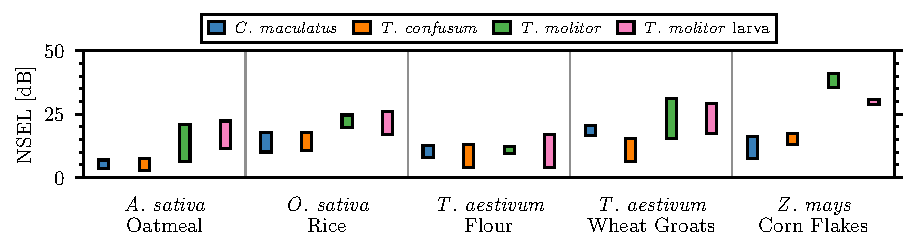
\includegraphics[width=\textwidth]{figures/nspa_nsel/nsel_box.pdf}
		\caption{Normalized Spectral Energy Level (NSEL)}
		\label{fig:nsel_box}
	\end{subfigure}

	\caption{Normalized Signal Pulse Amplitude (NSPA) and Normalized Spectral Energy Level (NSEL) for different insect species in various materials}%
	\label{fig:nspa_nsel}
\end{figure}

\newpage

Table \ref{tab:nspa_nsel_comparison} details the averaged values of the metrics

\begin{table}[!htbp]
	\centering
    \small
	\begin{tabularx}{\linewidth}{llrrrrr}
		\toprule
		                    &                           & \textbf{\textit{A. sativa}} & \textbf{\textit{O. sativa}} & \multicolumn{2}{c}{\textbf{\textit{T. aestivum}}} & \textbf{\textit{Z. mays}}               \\
		                    &                           & Oatmeal                        & Rice                           & Flour                                                   & Wheat Groats               & Corn Flakes \\
		\midrule
		\multirow{4}*{NSPA} & \textit{C. maculatus}     & 39.7                           & 46.2                           & 42.6                                                    & 58.4                       & 49.3        \\
		                    & \textit{T. confusum}      & 35.4                           & 45.9                           & 39.5                                                    & 43.9                       & 53.9        \\
		                    & \textit{T. molitor}       & 45.6                           & 62.7                           & 42.5                                                    & 60.1                       & 70.3        \\
		                    & \textit{T. molitor} larva & 56.8                           & 56.8                           & 39.6                                                    & 61.0                       & 70.5        \\
		\midrule
		\multirow{4}*{NSEL} & \textit{C. maculatus}     & 9.9                            & 17.3                           & 12.4                                                    & 24.2                       & 14.4        \\
		                    & \textit{T. confusum}      & 7.4                            & 18.2                           & 12.8                                                    & 13.0                       & 17.3        \\
		                    & \textit{T. molitor}       & 16.5                           & 32.8                           & 15.5                                                    & 28.3                       & 38.4        \\
		                    & \textit{T. molitor} larva & 23.1                           & 25.9                           & 11.2                                                    & 29.5                       & 34.8        \\ \bottomrule
	\end{tabularx}
	\caption{Comparison of NSPA and NSEL for different insect species}
	\label{tab:nspa_nsel_comparison}
\end{table}

Figure \ref{fig:nspa_nsel} shows that in the majority of the tested commodities, the strongest signal amplitudes and energy were observed for the larger insects \textit{T. molitor} and its larval form. Small insects produced much smaller signals. The exception to this relationship was within flour, where all tested insects generated similar relatively low signals. This can be attributed to the specifics of the small particle vibration under the actions of the moving insects. Visual observation of the insects moving in the flour showed that the larger insects had difficulty moving in the material, frequently coating themselves and getting stuck in the powder. A theoretical model describing the vibration and sound generation by insects in material was not found in any publication and might be a subject for future research.

\newpage
\subsection{Extending Analysis to BugBytes Dataset}

The derived approach can be extended to stored product insect data collected from other sensors including the BugBytes dataset which contains recordings from a piezoelectric disc sensor of a single \textit{Plodia interpunctella} larva in dry dog food and multiple \textit{S. oryzae} larvae in wheat groats. The recording system is not described in the dataset documentation but previous publications by the authors suggest that during recordings insects were placed directly on the piezoelectric disc sensor so the distance could not exceed \SI{1}{\milli\meter} \cite{mankinAcousticIndicatorsTargeted2010}.

The median normalization method was applied to the recordings from the ``Stored Product Insect movement and feeding sounds recorded for insect detection and monitoring studies'' portion of the BugBytes dataset to accommodate for the absense of any recordings without an insect to use as a reference self-noise signal. The recordings include single larva and multiple larvae of the \textit{Plodia interpunctella} in dry dog food, multiple larvae of the \textit{Sitophilus oryzae} larvae in wheat groats, multiple \textit{Sitophilus zeamais} adults and larvae in maize, and multiple \textit{Prostephanus truncatus} adults and larvae in maize. The sensors featured accelerometers, piezoelectric discs, Polyvinylidene difluoride (PVDF) sensors, ultrasonic sensors, and microphones.

The \textit{Sitophilus oryzae}, lesser grain borer or rice weevil, larvae are internal feeders and develop while
feeding within the grain. The larvae are \SIrange{1}{4}{\milli\meter} in length and are similar in size to the smaller insects recorded with the A-SPIDS \cite{cabiSitophilusOryzaeLesser2021}. Figure \ref{fig:sitophilus characteristics} shows a spectrogram and spectra recorded by a piezoelectric disc sensor of the \textit{Sitophilus oryzae}, the rice weevil, larvae in wheat groats from the BugBytes dataset. 

\begin{figure}[!htbp]
	\centering
	\begin{subfigure}{\textwidth}
		\centering
		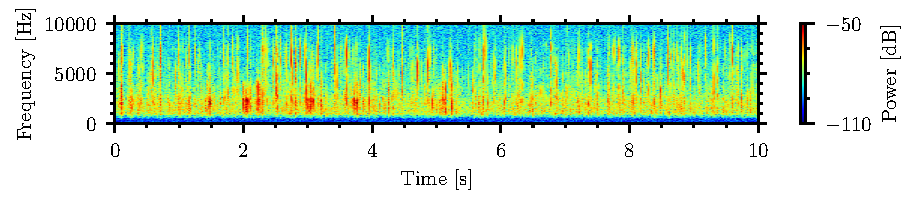
\includegraphics[width=\textwidth]{figures/bug_bytes/piezoelectric - Sitophilus oryzae_spectrogram.pdf}
		\caption{Spectrogram}
		\label{fig:sitophilus spectrogram}
	\end{subfigure}
	\qquad
	\begin{subfigure}{\textwidth}
		\centering
		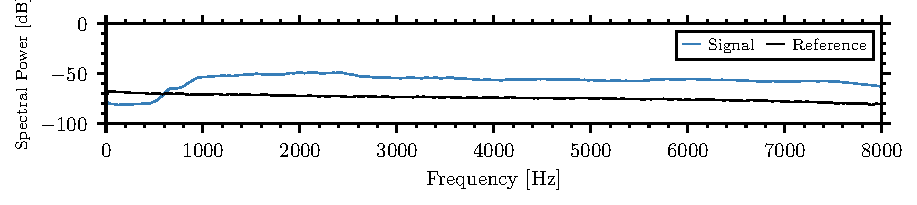
\includegraphics[width=\textwidth]{figures/bug_bytes/piezoelectric - Sitophilus oryzae_spectra.pdf}
		\caption{Spectra}
		\label{fig:sitophilus spectra}
	\end{subfigure}
	\caption{\textit{S. oryzae} larvae in wheat groats recorded by the piezoelectric sensor from the BugBytes dataset}%
	\label{fig:sitophilus characteristics}
\end{figure}

% \begin{figure}[!htbp]
% 	\centering
% 	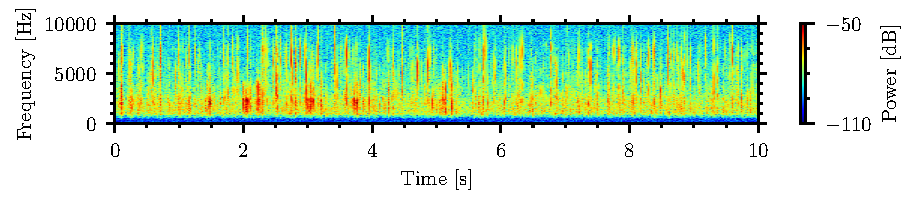
\includegraphics[width=\textwidth]{figures/bug_bytes/piezoelectric - Sitophilus oryzae_spectrogram.pdf}
% 	\caption{Spectrogram of \textit{Sitophilus oryzae} larvae in wheat groats recorded by the piezoelectric sensor from the BugBytes dataset}
% 	\label{fig:sitophilus spectrogram}
% \end{figure}

% Similarly to the recordings made by the A-SPIDS sensor, the BugBytes recording also features the impulses generated by the insect presence. These impulses are greatest in magnitude from \SIrange{500}{8000}{\hertz} and this frequency range was chosen for the median normalization method as well as NSPA and NSEL calculations. 

% \newpage
% Figure \ref{fig:sitophilus spectra} shows the spectra of the multiple \textit{Sitophilus oryzae}, the rice weevil, larvae in wheat groats:

% \begin{figure}[!htbp]
% 	\centering
% 	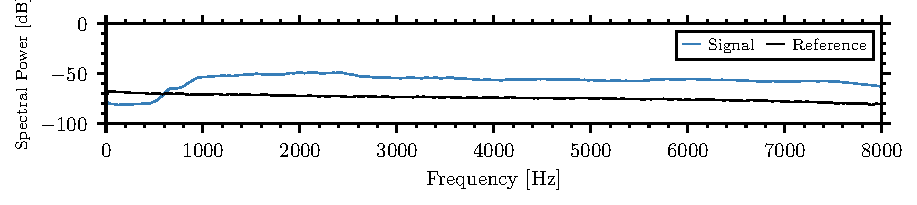
\includegraphics[width=\textwidth]{figures/bug_bytes/piezoelectric - Sitophilus oryzae_spectra.pdf}
% 	\caption{Spectra of \textit{Sitophilus oryzae} larvae in wheat groats recorded by the piezoelectric sensor from the BugBytes dataset}
% 	\label{fig:sitophilus spectra}
% \end{figure}

\newpage
The BugBytes recording also features the impulses generated by the insect presence. The frequency range of \SIrange{500}{8000}{\hertz} was chosen for the median normalization method as well as NSPA and NSEL calculations. Figure \ref{fig:sitophilus envelope} shows the normalized envelope of the \textit{S. oryzae}, the rice weevil, larvae in wheat groats with the highlighted NSPA analysis region and calculated value. The NSPA measurement of the \textit{S. oryzae} larvae in wheat groats was calculated to be \SI{37.49}{\decibel} and the NSEL measurement was \SI{19.43}{\deci\bel}. These values are comparable to the smaller insects in the same material from the A-SPIDS data. The NSPA values were calculated for the other recordings in the BugBytes dataset and are presented in Table \ref{tab:bugbytes}.

\begin{figure}[!htbp]
	\centering
	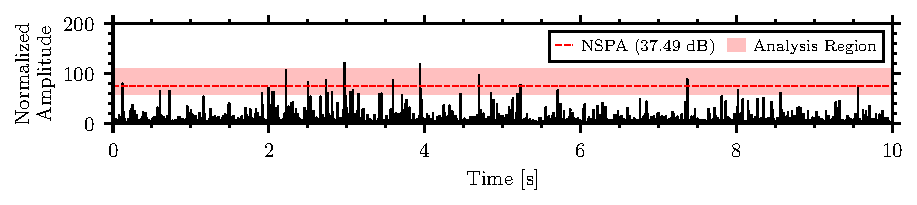
\includegraphics[width=\textwidth]{figures/bug_bytes/piezoelectric - Sitophilus oryzae_envelope.pdf}
	\caption{Normalized filtered envelope of \textit{S. oryzae} larvae in wheat groats recorded by the piezoelectric sensor from the BugBytes dataset}
	\label{fig:sitophilus envelope}
\end{figure}



\begin{table}[!htbp]
	\caption{NSPA of the stored product insect-material pairing recordings available in the BugBytes dataset \label{tab:bugbytes}}
	\centering
    \small
	\begin{tabular}{llllrr}
		\toprule
		\textbf{Subject}           & \textbf{Stage} & \textbf{Material} & \textbf{Sensor}                 & \textbf{Band} [\si{\hertz}] & \textbf{NSPA} [\si{\deci\bel}] \\ \midrule
		\textit{P. interpunctella} & Larvae         & Dog Food          & Accelerometer                   & 2000-3000                   & 32.97                          \\
		\textit{P. interpunctella} & Larva          & Dog Food          & Piezoelectric                   & 400-1200                    & 30.79                          \\
		\textit{S. oryzae}         & Larvae         & Wheat Groats      & PVDF film                       & 4000-11000                  & 38.15                          \\
		\textit{S. oryzae}         & Larvae         & Wheat Groats      & Accelerometer                   & 2500-10000                  & 42.57                          \\
		\textit{S. oryzae}         & Larvae         & Wheat Groats      & \SI{30}{\kilo\hertz} Ultrasonic & 2000-6000                   & 11.74                          \\
		\textit{S. oryzae}         & Larvae         & Wheat Groats      & \SI{40}{\kilo\hertz} Ultrasonic & 6000-9000                   & 24.70                          \\
		\textit{S. oryzae}         & Larvae         & Wheat Groats      & Piezoelectric                   & 500-8000                    & 37.49                          \\
		\textit{S. zeamais}        & Larvae         & Maize             & Microphone                      & 1000-4000                   & 22.35                          \\
		\textit{S. zeamais}        & Adults         & Maize             & Microphone                      & 1000-6000                   & 38.21                          \\
		\textit{P. trancatus}      & Larvae         & Maize             & Microphone                      & 1000-8000                   & 36.72                          \\
		\textit{P. trancatus}      & Adults         & Maize             & Microphone                      & 1000-8000                   & 29.67                          \\ \bottomrule
	\end{tabular}
\end{table}

The results of the NSPA analysis demonstrated the effectivity of using the median normalization method to compare insects signals across different sensors and materials. The results from the piezoelectric sensors of the BugBytes dataset are similar to the value ranges of the A-SPIDS sensor, but the A-SPIDS sensor was able to detect single at distances beyond \SI{10}{\centi\meter} with a higher sensitivity. Although the adult stage of the \textit{S. zeamais} had higher NSPA values than its larval stage, the opposite was observed for the \textit{P. truncatus} adults and larvae. Recordings of the \textit{S. oryzae} larvae in wheat groats across the different sensors revealed that the accelerometer had the highest sensitivity, followed by the PVDF film sensor, the piezoelectric sensor, and the ultrasonic sensors. Although the \SI{30}{\kilo\hertz} ultrasonic sensor was observed to have the lowest sensitivity, smaller than its \SI{40}{\kilo\hertz} counterpart, the insects could have been less active during the recording \cite{mankinAcousticIndicatorsTargeted2010}. 
% The little amount of recorded data in the BugBytes dataset does not allow for greater statistical comparison of the sensors or further generalization of acoustic insect signatures, but the results are consistent with other publications \cite{mankinAcousticIndicatorsTargeted2010}.

\newpage